\documentclass[11pt,a5paper]{article}
\usepackage[utf8]{inputenc}
\usepackage[english]{babel}
\usepackage{amsmath}
\usepackage{graphicx}
\usepackage{amsthm}
\usepackage{amsfonts}
\usepackage[margin=0.47in]{geometry}

\newtheorem{theorem}{}
\newtheorem{definition}{Definition}
\newtheorem{exercise}{Exercise}
\newtheorem{problem}{Problem}
\newtheorem*{corollary}{Corollary}

\makeatletter
\newenvironment{chapquote}[2][2em]
  {\setlength{\@tempdima}{#1}%
   \def\chapquote@author{#2}%
   \parshape 1 \@tempdima \dimexpr\textwidth-2\@tempdima\relax%
   \itshape}
  {\par\normalfont\hfill--\ \chapquote@author\hspace*{\@tempdima}\par\bigskip}
\makeatother

\title{\textbf{Sets and Infinity}}
\date{Weeks 3 \& 4}
\author{Miroslav Stankovic\\}
\begin{document}
\maketitle


\section{Naive Set Theory}

The idea of infinity have always been part of mathematics and philosophy. It has been part of fameous Zeno's paradoxes, infinite lines in geometry, or basis of analysis in the times of Leibnitz and Newton. However, until late 18th century, the infinity was viewed as something indefinite - as a limit, towards which a variable goes.

\begin{definition}
By a \emph{set} we understand any collection into a whole $M$ of definite and separate objects $m$ of our intuition or our thought. These objects are called the \emph{elements} of $M$.
\end{definition}

\noindent The definition above was used by Georg Cantor to establish the foundations of set theory, which allowed, for the first time, to directly work with infinity. As you may notice, the Cantor's definition lack the precision and rigour we are used to. In 1901, Bertrand Russel came up with a paradox in the Cantor's set theory. It goes like this: $S=\{x|x\notin x\}$.

\begin{exercise} 
What is the Russel's paradox about?
\end{exercise}

\noindent Cantor's set theory was later 'fixed' using mathematical logic and rigorous axiomatic approach to study sets. For the time being, the naive set theory will be sufficient to demonstrate basic concepts in infinities.

\section{Infinities}

\noindent In set theory, Cantor's diagonal argument was published in 1891 as a mathematical proof that there are infinite sets which cannot be put into one-to-one correspondence with the infinite set of natural numbers. Such sets are now known as uncountable sets, and the size of infinite sets is now treated by the theory of cardinal numbers which Cantor began. 

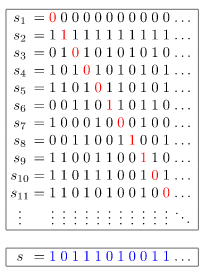
\includegraphics[scale=0.8]{cda}

\begin{exercise}
Let $S=\{x|x\subset \mathbb{N}\}$. Show that there is no bijection from $\mathbb{N}$ to $S$.
\end{exercise}

\begin{corollary} 
There are infinities of different sizes.
\end{corollary}

\begin{problem} 
Can Cantor's diagonal argument be used to prove existence of sets bigger than $\mathbb{R}$?
\end{problem}

\subsection*{Comparing infinities}

\noindent So how to compare two infinite sets? We can try to pair the elements, and if we are successful the sets are same size; if some elements are left umpired in a set, that set is bigger. Based on this idea we use following definition:

\begin{definition}
$A\preceq B$ if there is an injective function from $A$ to $B$;

$A\approx B$ if there is a bijection from $A$ to $B$; 

$A\prec B$ if $A\preceq B$ and $A\not\approx B$.
\end{definition}


\noindent There are several obvious properties of $\preceq, \approx, \prec$.
\begin{enumerate}
  \item $A\approx A$
  \item $A\approx B \Rightarrow B\approx A$
  \item If $A\approx B$ and $B\approx C$ then $A\approx C$
  \item If $A\preceq B$ and $B\preceq C$ then $A\preceq C$
  \item If $A\approx B$ then $A\preceq B$ and $B\preceq A$
\end{enumerate}

\noindent You might be surprised, that following (very plausible) property is missing: $A\preceq B$ and $B\preceq A$ then $A\approx B$. Even though it is true, it is not at all obvious! This theorem is known as Cantor-Bernstein theorem.

\begin{problem} 
Prove the Cantor-Bernstein theorem.
\end{problem}

\begin{exercise} 
Show that $(0,1)\approx\mathbb{R}$.
\end{exercise}

\subsection*{Finite vs. infinite}

\noindent Let's look at the following properties of finite sets.
\begin{enumerate}
  \item If $A$ is finite and $a \not\in A$ then $A\prec (A\cup \{a\})$.
  \item If $A$ is finite and $B\subset A$ then $B\prec A$.
  \item If $A$ is finite with at least two elements then $A \prec A\times A$ .
\end{enumerate}

\noindent However, none of these 'obvious' statements are true for infinite sets. Take $A\approx \mathbb{N}$. Then $\mathbb{N} \approx \mathbb{N}\cup \{0\}$ - we can take bijection $f(x) = x+1$. If $B$ is set of even natural numbers, then $B\subset A$ but $B\approx A$ thanks to bijection $f(x) = x/2$. And finaly:
\begin{exercise}
Show that $\mathbb{N} \approx \mathbb{N} \times \mathbb{N}$.
\end{exercise}

\noindent So even if cartesian product creates, in some sense, much bigger set, it is still the same countable infinity. In fact, $A\approx A\times A$ for any infinite set $A$. As a consequence, $A\approx A^n$ for any $n\in \mathbb{N}$. Another way how to create 'bigger' sets is using union - and since today it is all about infinity, let it be infinite union!

\begin{theorem}
Countable union of countable sets is countable.
\end{theorem}

\begin{proof} 
Consider the countable sets $S_0, S_1, S_2, \ldots$ where $\displaystyle S = \bigcup_{i \mathop \in \mathbb{N}} {S_i}$. Now we write the elements of $S_0, S_1, S_2, \ldots$ in the form of a table:

$\begin{array} {*{4}c} {a_{00}} & {a_{01}} & {a_{02}} & \cdots \\ {a_{10}} & {a_{11}} & {a_{12}} & \cdots \\ {a_{20}} & {a_{21}} & {a_{22}} & \cdots \\ \vdots & \vdots & \vdots & \ddots \\ \end{array}$

\noindent where $a_{ij}$ is the $j$th element of set $S_i$. This table clearly contains all the elements of $\displaystyle S = \bigcup_{i \mathop \in \mathbb{N}} {S_i}$, so we have $S \approx \mathbb{N}\times\mathbb{N} \approx \mathbb{N}$.
\end{proof}

\begin{exercise} Using Cantor-Bernstein theorem, show that $\mathbb{Q}\approx\mathbb{N}$. 
\end{exercise}

\begin{problem} 
Show that $\mathbb{R} \approx \mathbb{N} \times \mathbb{R}$.
\end{problem}

\begin{problem} 
Show that $\mathbb{R} \approx \mathbb{R} \times \mathbb{R}$.
\end{problem}

\begin{problem} 
Show that set of all finite subsets of $\mathbb{N}$ is countable.
\end{problem}

\begin{problem} 
Show that set of all finite subsets of $\mathbb{N}$ is countable.
\end{problem}

\noindent So far we have looked at the sets as some abstract structures. However, we can represent $\mathbb{R}$ simply as a line, $\mathbb{R}\times\mathbb{R}$ as a plane, infinite square grid as a $\mathbb{N}\times\mathbb{N}$, and so on. In the following examples, try to use intuitive, geometrical approach.

\begin{enumerate}
  \item Show that $(0,\pi)\approx\mathbb{R}$
  \item Show that 'unit square' $\approx\mathbb{R}^2$.
  \item How many lines do we need to cover a plane?
  \item Can we color all squares in infinite square grid with two colors (green and blue) such that every column contains finitly many green squares, and every row finitely many blue squares?
\end{enumerate}

\section{Axiomatic set theory}

Several systems of axioms were developed to get rid of the paradoxes in naive set theory. The most common one is Zermelo-Fraenkel Axioms, so called ZF.

\begin{enumerate}
	\item \emph{Axiom of extensionality}: 
Two sets are equal (are the same set) if they have the same elements.
\[\forall x \forall y [ \forall z (z \in x \Leftrightarrow z \in y) \Rightarrow x = y]\]

	\item \emph{Axiom of regularity}:
Every non-empty set $x$ contains a member $y$ such that $x$ and $y$ are disjoint sets.
\[\forall x [ \exists a ( a \in x) \Rightarrow \exists y ( y \in x \land \lnot \exists z (z \in y \land z \in x))]\]
\begin{exercise}
Show that Axiom of regularity get rid of Russel's paradox.
\end{exercise}

	\item \emph{Axiom schema of specification}:
Essentially, it says that any definable subclass of a set is a set, i.e. for any $X$ and parameter $p$, there is a set $\{x \in X : \phi(x,p)\}$.
\[\forall z \forall p \exists y \forall x [x \in y \Leftrightarrow ( x \in z \land \phi(x,p) )]\]

	\item \emph{Axiom of pairing}:
If $x$ and $y$ are sets, then there exists a set which contains $x$ and $y$ as elements.
\[\forall x \forall y \exists z (x \in z \land y \in z)\]
	
	\item \emph{Axiom of union}:
The union over the elements of a set exists.
\[\forall \mathcal{F} \,\exists A \, \forall Y\, \forall x [(x \in Y \land Y \in \mathcal{F}) \Rightarrow x \in A\]
	
	\item \emph{Axiom schema of replacement}:
The axiom schema of replacement asserts that the image of a set under any definable function will also fall inside a set.
If $F$ is a function, then for any $X$ there exists a set $Y=F[X]=\{F(x):x \in X\}$.
	
	\item \emph{Axiom of infinity}:
	\[\exists X \left [\emptyset \in X \land (\forall y \in X )[x \cup \{x\}  \in X]\right ]\]
	
	\item \emph{Axiom of power set}:
The Axiom of Power Set states that for any set $x$, there is a set $y$ that contains every subset of $x$.
\[\forall x \exists y \forall z [z \subseteq x \Rightarrow z \in y]\]
	
\end{enumerate}

\section{Axiom of choice}

\noindent ZF is often extended by adding one extra axiom - the Axiom of Choice - to form so called ZFC system. Informally put, the axiom of choice, or simply AC, says that given any collection of bins, each containing at least one object, it is possible to make a selection of exactly one object from each bin.

\noindent More formaly: For any set X of nonempty sets, there exists a choice function f defined on X.
\\

\begin{chapquote}{Bertrand Russell, \textit{Introduction to mathematical philosophy}}
\noindent The Axiom of Choice is necessary to select a set from an infinite number of pairs of socks, but not an infinite number of pairs of shoes.
\end{chapquote}	

\noindent Axiom of choice, is one of most controversial axioms in mathematics. Although it seems perfectly obvious, it allows us to do some really weird stuff. With AC, it is possible to decompose a ball into a finite number of point sets and reassemble it into two balls identical to the original (Banach–Tarski paradox). 

\noindent There are several statements equivalent to the AC. \\

\noindent \emph{Zorn's lemma}: 
Suppose a partially ordered set P has the property that every chain (i.e. totally ordered subset) has an upper bound in P. Then the set P contains at least one maximal element.\\

\noindent \emph{Well-ordering theorem}: 
The well-ordering theorem states that every set can be well-ordered.\\

\begin{chapquote}{Jerry Bona}
\noindent The Axiom of Choice is obviously true, the well-ordering principle obviously false, and who can tell about Zorn's lemma?
\end{chapquote}	


\begin{problem}
150 logicians (labeled 1 through 100) were captured by an evil philosopher. He gives them some time to prepare a strategy and then let them stand in a row - so that everyone only sees people with higher number. Then they are all given a blue or a green hat (they do not know what color they got). Starting from \#1, each have to guess the color of their hat. Only those who guess correctly survive.
\begin{enumerate}
	\item What strategy should they use, to make sure at least 75 of them survive?
	\item How about at least 100?
	\item Or 149?
	\item How to make sure that at most one survive?
	\item What if C different colors are used?
\end{enumerate}
\end{problem}

\begin{problem}
This time, the evil philosopher captured countably many set theorists. Again, they have time to decide on a strategy and then they will go through the same process as logicians in the last problem. How can they make sure, that only finitely many of them do not survive?
\end{problem}

\begin{problem}
In a room, there is countably many envelopes, each containing a real number. One by one, 100 set theorists visit the room and each can open countably many of the envelopes. Then he or she have to pick an unopened envelope and guess what number is inside (after each visit, envelopes are returned to the original state). Can we guarantee that at least one of them guesses right? What about 99 correct guesses?
\end{problem}

\end{document}

\\https://mks.mff.cuni.cz/common/show.php?title=Nekone%26%23269%3Bn%26eacute%3B+mno%26%23382%3Biny&file=library/NekonecneMnozinyDS/NekonecneMnozinyDS
\\https://mks.mff.cuni.cz/common/show.php?title=Teorie+mno%26%23382%3Bin&file=library/TeorieMnozinPPo/TeorieMnozinPPo
\\https://en.wikipedia.org/wiki/Cantor%27s_diagonal_argument
\\https://mks.mff.cuni.cz/library/AGNerovnostLZ/AGNerovnostLZ.pdf
\\https://en.wikipedia.org/wiki/Axiom_of_choice
